\chapter{कोशिकीय श्वसन और किण्वन}\label{ch:g12:respiration-fermentation}

किसी मैराथन धावक की पेशियाँ साढ़े तीन घंटों पर हर मिनट लगभग आधा मोल \omterm{def:g12:respiration-fermentation:atp}{ATP}
ख़र्च करती हैं --- यानी उस अणु का एक चौथाई किलोग्राम, जो ऐसे भंडार से हज़ारों
बार बनाया, इस्तेमाल किया और दोबारा बनाया जाता है जो पाँच सेकंड चलता।
उनमें से हर \omterm{def:g12:respiration-fermentation:atp}{ATP} अणु की क़ीमत कोई ग्लूकोज या कोई वसीय अम्ल चुकाता है, जिसे
परमाणु दर परमाणु तोड़ा जाता है, और वह ऑक्सीजन अणु भी जो शुरू में साँस के
साथ भीतर लिया जाता है और आख़िर में पानी की तरह बाहर।
\cref{ch:g10:cell-metabolism} ने संतुलन दिया था; यह अध्याय \omterm{def:g10:cells-common-unit:organelle}{सूत्रकणिका} खोलता
है और उन तीन चरणों से होकर ग्लूकोज का पीछा करता है जो उसकी ऊर्जा को \omterm{def:g12:respiration-fermentation:atp}{ATP} में
बदलते हैं --- और दिखाता है कि ऑक्सीजन चुक जाए तो कोई \omterm{def:g10:cells-common-unit:cell}{कोशिका} क्या करती है।

\section{ATP, वह मुद्रा}

\begin{definition}[ATP]\label{def:g12:respiration-fermentation:atp}
\emph{ATP}\index{ATP} (एडिनोसीन ट्राइफ़ॉस्फ़ेट) एक \omterm{def:g10:universal-dna:nucleotide}{न्यूक्लियोटाइड} है जो
क़तार में तीन फ़ॉस्फ़ेट समूह ढोता है। आख़िरी को हटाने पर \omterm{def:g10:cells-common-unit:cell}{कोशिका} की
परिस्थितियों में प्रति मोल लगभग \qty{30}{kJ} छूटते हैं, और \omterm{def:g10:cells-common-unit:cell}{कोशिका} की हर
ऊर्जा माँगती प्रक्रिया --- संकुचन, परिवहन, संश्लेषण, किसी जुगनू की रोशनी ---
उसी हटाव से चलती है। उसका उत्पाद, ADP, इस अध्याय की अभिक्रियाओं से दोबारा
ATP में चार्ज होता है। कोई \omterm{def:g10:cells-common-unit:cell}{कोशिका} कुछ ही सेकंड लायक़ ATP थामती है और उसे
लगातार पलटती रहती है; और विश्राम करता कोई मनुष्य एक दिन में लगभग अपने ही
शरीर के द्रव्यमान भर ATP पुनर्चक्रित करता है।
\end{definition}

\begin{proposition}[ऊर्जा कहाँ है]\label{prop:g12:respiration-fermentation:oxidation}
ग्लूकोज अपने कार्बन--हाइड्रोजन बंधों में ऊर्जा जमा रखता है; और उसे छोड़ने
का मतलब है उस हाइड्रोजन को, उसके इलेक्ट्रॉनों समेत, ऑक्सीजन तक पहुँचाना ---
यानी ग्लूकोज को कार्बन डाइऑक्साइड तक ऑक्सीकृत करना और ऑक्सीजन को पानी तक
अपचयित। किसी लौ की तरह एक ही क़दम में किया जाए तो वह ऊर्जा ऊष्मा की तरह
निकल जाती। \omterm{def:g10:cells-common-unit:cell}{कोशिका} उसे दर्जनों छोटे क़दमों में करती है, जिनमें से हर एक कोई
\omterm{def:g11:enzymes-and-phenotype:enzyme}{एंजाइम} चलाता है, और उनमें से कई पर ऊर्जा का एक हिस्सा पकड़ लेती है: वह
हाइड्रोजन पहले वाहक अणुओं --- यानी \emph{अपचयित NAD} --- पर लादा जाता है,
और केवल आख़िर में ऑक्सीजन को सौंपा जाता है।
\end{proposition}
\admitted

\section{तीन चरण}

\begin{proposition}[ग्लाइकोलिसिस]\label{prop:g12:respiration-fermentation:glycolysis}
\omterm{def:g10:cells-common-unit:cell}{कोशिकाद्रव्य} में, बिना ऑक्सीजन के, कोई ग्लूकोज (छह कार्बन) दस \omterm{def:g11:enzymes-and-phenotype:enzyme}{एंजाइम}
क़दमों से \emph{पाइरुवेट} (हर एक तीन कार्बन) के दो अणुओं में चीर दिया जाता
है: यानी \emph{ग्लाइकोलिसिस}\index{ग्लाइकोलिसिस}। संतुलन: शुरू करने को दो
\omterm{def:g12:respiration-fermentation:atp}{ATP} खपे, चार बने, यानी 2 \omterm{def:g12:respiration-fermentation:atp}{ATP} का शुद्ध लाभ, और हाइड्रोजन से लदे दो अपचयित
NAD। वह पाइरुवेट अब भी ग्लूकोज की अधिकांश ऊर्जा थामे है।
\end{proposition}
\admitted

\begin{proposition}[सूत्रकणिका उस ऑक्सीकरण को पूरा करती है]\label{prop:g12:respiration-fermentation:mitochondrion}
ऑक्सीजन उपलब्ध हो तो पाइरुवेट \emph{सूत्रकणिका}\index{सूत्रकणिका} में घुसता
है, जो दो झिल्लियों से घिरा एक \omterm{def:g10:cells-common-unit:organelle}{कोशिकांग} है, और जिसकी भीतरी झिल्ली
\emph{क्रिस्टी} में मुड़ी है तथा तरल \emph{आधात्री} को घेरती है।
\begin{itemize}
  \item आधात्री में हर पाइरुवेट अभिक्रियाओं के एक चक्र में, यानी
        \emph{क्रेब्स चक्र}\index{क्रेब्स चक्र} में, तोड़ा जाता है: उसके
        तीनों कार्बन तीन $\mathrm{CO_2}$ की तरह निकलते हैं, उसका हाइड्रोजन
        वाहकों पर लादा जाता है (अपचयित NAD और एक दूसरा वाहक), और थोड़ा \omterm{def:g12:respiration-fermentation:atp}{ATP}
        सीधे बनता है --- प्रति पाइरुवेट एक।
  \item भीतरी झिल्ली में वे लदे वाहक अपने इलेक्ट्रॉन प्रोटीनों की एक
        शृंखला को सौंपते हैं, यानी \emph{श्वसन शृंखला} को, जो उन्हें नीचे
        ऑक्सीजन तक पहुँचाती है, और वह प्रोटॉनों से जुड़कर पानी बनाती है।
        उस शृंखला पर छूटती ऊर्जा प्रोटॉनों को उस झिल्ली के पार पंप करती है,
        और किसी घूमते \omterm{def:g11:enzymes-and-phenotype:enzyme}{एंजाइम} से होकर उनकी वापसी \omterm{def:g12:respiration-fermentation:atp}{ATP} का संश्लेषण चलाती है
        --- यानी प्रति ग्लूकोज लगभग 26।
\end{itemize}
एक ग्लूकोज के लिए कुल: लगभग 30 \omterm{def:g12:respiration-fermentation:atp}{ATP} (2 \omterm{prop:g12:respiration-fermentation:glycolysis}{ग्लाइकोलिसिस} से, 2 उस चक्र से, कोई 26
उस शृंखला से), छह $\mathrm{CO_2}$ छोड़ी गईं, छह $\mathrm{O_2}$ खपीं, और
\qty{2870}{kJ} का बाक़ी हिस्सा ऊष्मा की तरह।
\end{proposition}
\begin{proof}[साक्ष्य]
किसी बंद कक्ष में ऑक्सीजन जाँच के साथ रखी अलग की गई \omterm{def:g10:cells-common-unit:organelle}{सूत्रकणिकाएँ} ग्लूकोज
देने पर कोई ऑक्सीजन नहीं खपातीं, पर पाइरुवेट देने पर उसे तेज़ी से खपाती हैं
--- यानी \omterm{def:g10:cells-common-unit:organelle}{सूत्रकणिका} ग्लूकोज से शुरू नहीं कर सकती; \omterm{def:g10:cells-common-unit:cell}{कोशिकाद्रव्य} को करना पड़ता
है। श्वसन शृंखला का कोई ज़हर (साइनाइड) जोड़ने पर वह खपत तुरंत रुक जाती है,
चाहे कोई भी \omterm{def:g11:enzymes-and-phenotype:enzyme}{क्रियाधार} मौजूद हो। ADP जोड़ने पर वह खपत तेज़ होती है और उसके
चुकने पर धीमी: यानी ऑक्सीजन का इस्तेमाल \omterm{def:g12:respiration-fermentation:atp}{ATP} संश्लेषण से जुड़ा है। और किसी
हमिंगबर्ड की उड़ान पेशी या किसी मैराथन धावक की जाँघ की \omterm{def:g10:cells-common-unit:organelle}{सूत्रकणिकाओं} में
क्रिस्टी किसी विश्राम करते ऊतक से कई गुना सघन भरी होती हैं।
\end{proof}

\begin{omfigure}
\begin{tikzpicture}
  \node[anchor=south west, inner sep=0] (img) at (0,0)
    {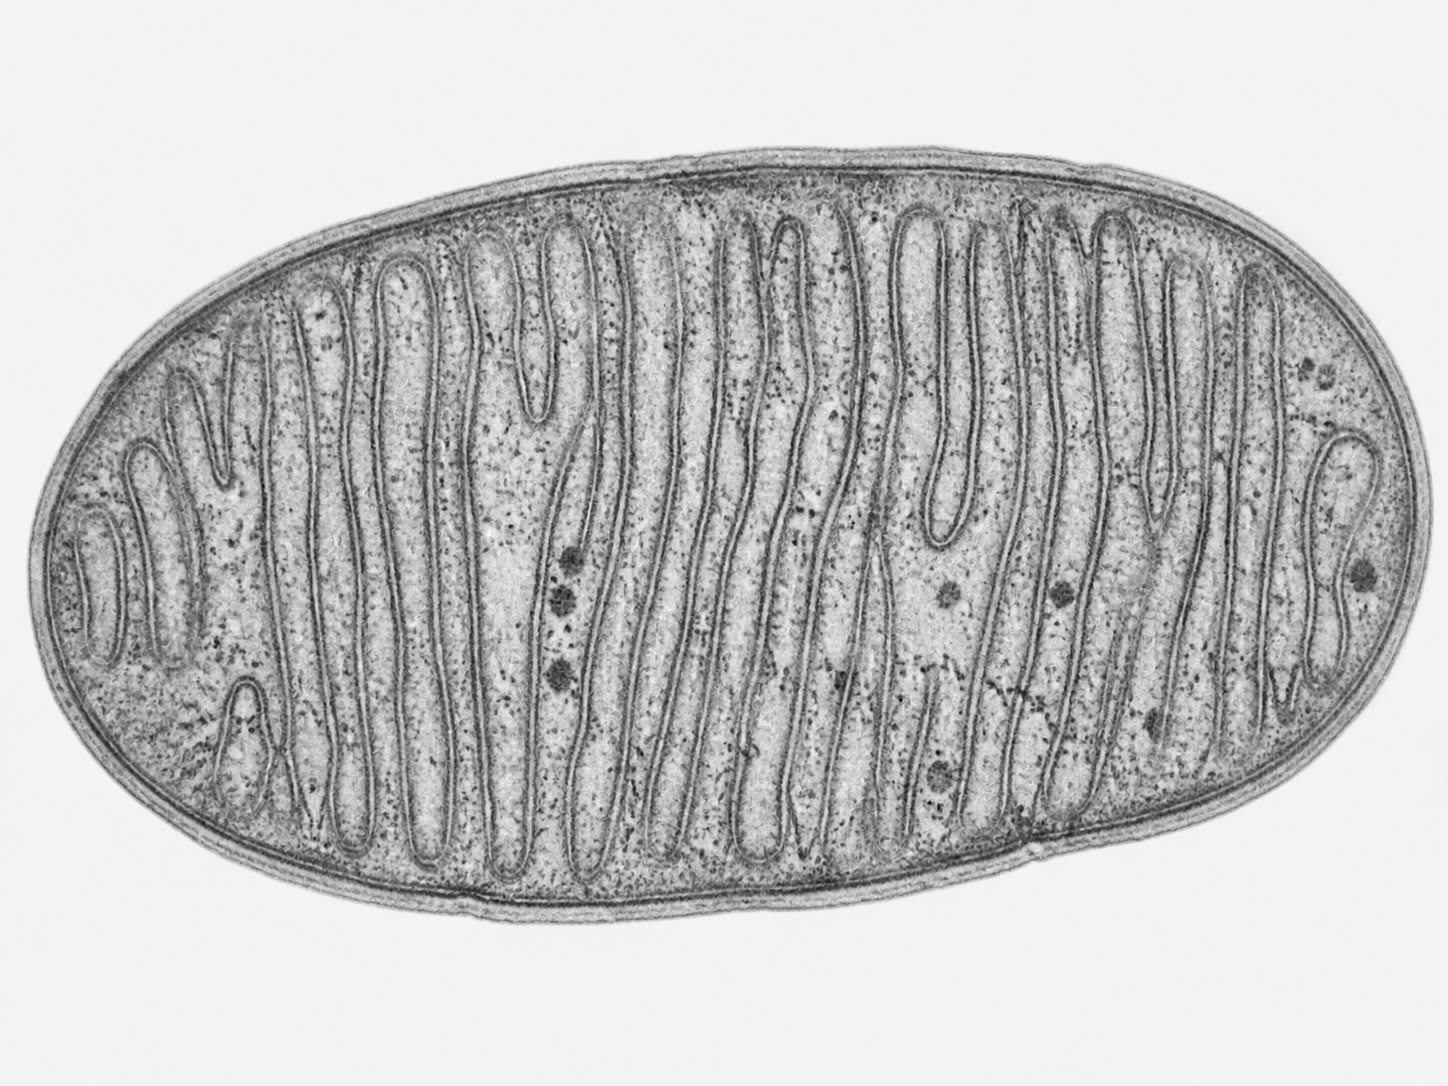
\includegraphics[width=0.5\linewidth]{images/book2/ai/g12-resp-mitochondrion-tem.jpg}};
  \begin{scope}[x={(img.south east)}, y={(img.north west)},
      every node/.style={font=\small}]
    \draw[omDef, thick] (0.08,0.55) -- (-0.04,0.80) node[left, align=right] {बाहरी\\ झिल्ली};
    \draw[omDef, thick] (0.20,0.45) -- (-0.04,0.25) node[left, align=right] {भीतरी झिल्ली,\\ क्रिस्टी में मुड़ी};
    \draw[omDef, thick] (0.55,0.50) -- (0.55,-0.06) node[below] {आधात्री (क्रेब्स चक्र)};
    \draw[omDef, thick] (0.80,0.60) -- (1.04,0.80) node[right, align=left] {क्रिस्टी: वह\\ श्वसन शृंखला};
  \end{scope}
\end{tikzpicture}

{\small इलेक्ट्रॉन सूक्ष्मदर्शी में एक \omterm{def:g10:cells-common-unit:organelle}{सूत्रकणिका}। भीतरी झिल्ली क्रिस्टी में
मुड़ी है, जो श्वसन शृंखला और \omterm{def:g12:respiration-fermentation:atp}{ATP} बनाता \omterm{def:g11:enzymes-and-phenotype:enzyme}{एंजाइम} ढोती हैं; और उनके बीच का
तरल, यानी आधात्री, \omterm{prop:g12:respiration-fermentation:mitochondrion}{क्रेब्स चक्र} चलाता है।}
\end{omfigure}

\begin{omfigure}
\begin{tikzpicture}[font=\small, >=Stealth,
  b/.style={draw, rounded corners, align=center, minimum height=0.9cm}]
  % cytoplasm region
  \node[b, fill=omDef!8, minimum width=6.0cm, minimum height=6.2cm] (cyt) at (0,0) {};
  \node[anchor=north, font=\small\bfseries] at (cyt.north) {कोशिकाद्रव्य};
  \node[b, fill=omMeth!20, text width=2.4cm] (glu) at (0,2.0) {ग्लूकोज (6 C)};
  \node[b, fill=omProp!20, text width=2.4cm] (pyr) at (0,-0.2) {2 पाइरुवेट\\ (हर एक 3 C)};
  \draw[->, thick] (glu) -- node[right, align=left, font=\scriptsize] {ग्लाइकोलिसिस:\\ $+2$ ATP, $+2$ NADH} (pyr);
  \node[b, fill=omThm!15, text width=2.6cm] (ferm) at (0,-2.4) {किण्वन:\\ लैक्टेट, या\\ इथेनॉल $+ \mathrm{CO_2}$};
  \draw[->, thick, omThm] (pyr) -- node[right, font=\scriptsize, align=left] {कोई $\mathrm{O_2}$ नहीं:\\ NADH दोबारा बना} (ferm);
  % mitochondrion region
  \node[b, fill=omProp!8, minimum width=6.4cm, minimum height=6.2cm, rounded corners=14pt] (mit) at (7.3,0) {};
  \node[anchor=north, font=\small\bfseries] at (mit.north) {सूत्रकणिका};
  \node[b, fill=omProp!20, text width=2.6cm] (krebs) at (7.3,1.4) {क्रेब्स चक्र\\ (आधात्री):\\ $6\,\mathrm{CO_2}$ बाहर,\\ $+2$ ATP, वाहक लदे};
  \node[b, fill=omThm!15, text width=2.8cm] (chain) at (7.3,-1.5) {श्वसन शृंखला\\ (भीतरी झिल्ली):\\ वाहक $+ \mathrm{O_2} \to \mathrm{H_2O}$,\\ $+26$ ATP};
  \draw[->, thick] (pyr.east) -- node[pos=0.72, above, font=\scriptsize] {$\mathrm{O_2}$ के साथ} (krebs.west |- pyr.east);
  \draw[->, thick] (krebs) -- node[right, font=\scriptsize] {अपचयित NAD} (chain);
  \draw[->, thick] (10.9,-1.1) -- (chain.east |- 0,-1.1) node[pos=0, right] {$6\,\mathrm{O_2}$};
  \draw[->, thick] (chain.east |- 0,-1.9) -- (10.9,-1.9) node[right] {$6\,\mathrm{H_2O}$};
  \draw[->, thick] (krebs.east |- 0,1.8) -- (10.9,1.8) node[right] {$6\,\mathrm{CO_2}$};
\end{tikzpicture}

{\small श्वसन के तीनों चरण, और \omterm{def:g10:cell-metabolism:fermentation}{किण्वन} वाला छोटा रास्ता। \omterm{def:g10:cells-common-unit:cell}{कोशिकाद्रव्य} में
\omterm{prop:g12:respiration-fermentation:glycolysis}{ग्लाइकोलिसिस} दो \omterm{def:g12:respiration-fermentation:atp}{ATP} तथा दो पाइरुवेट देता है; \omterm{def:g10:cells-common-unit:organelle}{सूत्रकणिका} में \omterm{prop:g12:respiration-fermentation:mitochondrion}{क्रेब्स चक्र}
उन्हें छीलकर कार्बन डाइऑक्साइड तक ले जाता है और वाहक लाद देता है, जिन्हें
श्वसन शृंखला ऑक्सीजन पर उतारती है तथा अधिकांश \omterm{def:g12:respiration-fermentation:atp}{ATP} बनाती है। बिना ऑक्सीजन के
पाइरुवेट \omterm{def:g10:cell-metabolism:fermentation}{किण्वन} की ओर मोड़ दिया जाता है, जो आगे कुछ नहीं देता।}
\end{omfigure}

\begin{example}[कोई ऑक्सीजन लेखा पढ़ना]\label{ex:g12:respiration-fermentation:trace}
कक्ष में अलग की गई \omterm{def:g10:cells-common-unit:organelle}{सूत्रकणिकाएँ}: ऑक्सीजन \qty{8}{mg/L} पर ठहरी रहती है;
ग्लूकोज जोड़ा जाता है, कुछ नहीं; पाइरुवेट जोड़ा जाता है, ऑक्सीजन प्रति मिनट
\qty{0.5}{mg/L} की दर से गिरती है; ADP जोड़ा जाता है, वह गिरावट कुछ देर के
लिए प्रति मिनट \qty{1.5}{mg/L} तक तीखी हो जाती है, फिर \num{0.5} पर लौट
आती है; साइनाइड जोड़ा जाता है, वह गिरावट रुक जाती है। एक ही लेखे में चार
तथ्य: \omterm{def:g10:cells-common-unit:organelle}{सूत्रकणिका} को पाइरुवेट चाहिए, ग्लूकोज नहीं; ऑक्सीजन का इस्तेमाल \omterm{def:g12:respiration-fermentation:atp}{ATP}
संश्लेषण से जुड़ा है; वह जुड़ाव उसी शृंखला से होकर है जिसे साइनाइड रोकता है;
और बिना काम की \omterm{def:g10:cells-common-unit:organelle}{सूत्रकणिका} सुस्त पड़ी रहती है।
\end{example}

\begin{omfigure}
\begin{tikzpicture}
\begin{axis}[
  width=0.9\linewidth, height=5.6cm,
  axis x line=bottom, axis y line=left,
  xmin=0, xmax=16, ymin=0, ymax=10,
  xlabel={समय (min)}, ylabel={घुली $\mathrm{O_2}$ (mg/L)},
  xlabel style={font=\small, at={(axis description cs:0.5,-0.12)}, anchor=north},
  ylabel style={font=\small},
  tick label style={font=\small}, xtick={0,2,4,6,8,10,12,14,16}, ytick={0,2,4,6,8},
  clip=false,
]
\addplot[thick, omThm] coordinates {(0,8) (2,8) (4,8) (6,7) (8,4) (10,3) (12,2) (14,2) (16,2)};
\draw[->, thick] (axis cs:2,9.6) -- (axis cs:2,8.4);
\node[font=\scriptsize, anchor=south] at (axis cs:2,9.7) {ग्लूकोज};
\draw[->, thick] (axis cs:4,9.6) -- (axis cs:4,8.4);
\node[font=\scriptsize, anchor=south] at (axis cs:4,9.7) {पाइरुवेट};
\draw[->, thick] (axis cs:6,9.6) -- (axis cs:6,8.4);
\node[font=\scriptsize, anchor=south] at (axis cs:6,9.7) {ADP};
\draw[->, thick] (axis cs:12,9.6) -- (axis cs:12,8.4);
\node[font=\scriptsize, anchor=south] at (axis cs:12,9.7) {साइनाइड};
\end{axis}
\end{tikzpicture}

{\small अलग की गई \omterm{def:g10:cells-common-unit:organelle}{सूत्रकणिकाओं} की ऑक्सीजन खपत। ग्लूकोज कुछ नहीं करता;
पाइरुवेट वह खपत शुरू करता है; ADP उसे तब तक तेज़ करता है जब तक वह ADP चुक न
जाए; और साइनाइड, जो श्वसन शृंखला रोकता है, उसे बंद कर देता है।}
\end{omfigure}

\section{बिना ऑक्सीजन के: किण्वन}

\begin{proposition}[किण्वन वाहक दोबारा बना देता है]\label{prop:g12:respiration-fermentation:fermentation}
\omterm{prop:g12:respiration-fermentation:glycolysis}{ग्लाइकोलिसिस} प्रति ग्लूकोज दो NAD वाहक लाद देता है; और ऑक्सीजन के साथ वह
\omterm{def:g10:cells-common-unit:organelle}{सूत्रकणिका} उन्हें उतार देती है। बिना ऑक्सीजन के वे सारे वाहक सेकंडों के भीतर
लदे रह जाते और \omterm{prop:g12:respiration-fermentation:glycolysis}{ग्लाइकोलिसिस} रुक जाता।
\emph{किण्वन}\index{किण्वन} \omterm{def:g10:cells-common-unit:cell}{कोशिकाद्रव्य} का उन्हें उतारने का ढंग है: वह
पाइरुवेट ख़ुद वह हाइड्रोजन ले लेता है और या तो \emph{लैक्टेट} बन जाता है
(पेशी \omterm{def:g10:cells-common-unit:cell}{कोशिकाएँ}, दूध के जीवाणु) या, कोई $\mathrm{CO_2}$ खोने के बाद,
\emph{इथेनॉल} (ख़मीर)। आगे कोई \omterm{def:g12:respiration-fermentation:atp}{ATP} नहीं बनता; पैदावार \omterm{prop:g12:respiration-fermentation:glycolysis}{ग्लाइकोलिसिस} के वही 2
\omterm{def:g12:respiration-fermentation:atp}{ATP} हैं, यानी श्वसन से कोई पंद्रह गुना कम, और वह उत्पाद --- लैक्टेट या
इथेनॉल --- अब भी ग्लूकोज की अधिकांश ऊर्जा थामे है।
\end{proposition}
\admitted

\begin{omfigure}
\begin{tikzpicture}
\begin{axis}[
  ybar, bar width=22pt,
  width=0.7\linewidth, height=5.2cm,
  axis x line=bottom, axis y line=left,
  ymin=0, ymax=36, ylabel={प्रति ग्लूकोज ATP},
  ylabel style={font=\small},
  symbolic x coords={किण्वन, ग्लाइकोलिसिस + क्रेब्स, पूरा श्वसन},
  xtick=data, tick label style={font=\small},
  enlarge x limits=0.3, ytick={0,10,20,30},
  nodes near coords, nodes near coords style={font=\small},
]
\addplot[fill=omThm!45, draw=omThm] coordinates {(किण्वन,2) (ग्लाइकोलिसिस + क्रेब्स,4) (पूरा श्वसन,30)};
\end{axis}
\end{tikzpicture}

{\small प्रति ग्लूकोज \omterm{def:g12:respiration-fermentation:atp}{ATP} पैदावार। अकेला \omterm{prop:g12:respiration-fermentation:glycolysis}{ग्लाइकोलिसिस}, अपने वाहक को दोबारा
बनाने के लिए \omterm{def:g10:cell-metabolism:fermentation}{किण्वन} के साथ, 2 देता है; \omterm{prop:g12:respiration-fermentation:mitochondrion}{क्रेब्स चक्र} सीधे 2 और जोड़ता है; और
श्वसन शृंखला, जिसे ऑक्सीजन चाहिए, बाक़ी 26 जोड़ती है।}
\end{omfigure}

\begin{example}[पेशी का चुनाव]\label{ex:g12:respiration-fermentation:muscle}
किसी फ़र्राटा धावक के \omterm{def:g10:muscles-and-joints:muscle}{पेशी तंतु} को \omterm{def:g12:respiration-fermentation:atp}{ATP} उससे तेज़ चाहिए जितना उसकी
\omterm{def:g10:cells-common-unit:organelle}{सूत्रकणिकाएँ} तथा उसकी ऑक्सीजन आपूर्ति बना सकें; लैक्टिक \omterm{def:g10:cell-metabolism:fermentation}{किण्वन} वाला
\omterm{prop:g12:respiration-fermentation:glycolysis}{ग्लाइकोलिसिस} \omterm{def:g12:respiration-fermentation:atp}{ATP} तीन गुना तेज़ पहुँचाता है, और वह भी पंद्रह गुनी ग्लूकोज
क़ीमत पर, तथा लैक्टेट तब तक जमा होता है जब तक दर्द उस मेहनत को रोक न दे।
किसी मैराथन धावक के तंतु श्वसन पर चलते हैं, धीरे और लगभग अनिश्चित काल तक,
और ग्लूकोज के साथ वसा भी जलाते हैं; उसकी \omterm{def:g10:cells-common-unit:organelle}{सूत्रकणिकाएँ} बड़ी तथा अधिक हैं,
उसकी केशिकाएँ सघन हैं, और उसका लैक्टेट नीचा रहता है।
\cref{ch:g10:muscles-and-joints} के तंतु प्रकार यही दो रणनीतियाँ हैं, जो
\omterm{def:g10:cells-common-unit:cell}{कोशिकाओं} में गढ़ी हैं।
\end{example}

\begin{method}[किसी ऊर्जा बजट का संतुलन]\label{met:g12:respiration-fermentation:budget}
\begin{enumerate}
  \item ज़रूरी शक्ति को \omterm{def:g12:respiration-fermentation:atp}{ATP} में बदलिए: प्रति मोल \omterm{def:g12:respiration-fermentation:atp}{ATP} लगभग \qty{30}{kJ}
        काम आती ऊर्जा पर, \qty{1}{kW} उपापचयी शक्ति प्रति मिनट
        \qty{2}{mol} \omterm{def:g12:respiration-fermentation:atp}{ATP} है।
  \item \omterm{def:g12:respiration-fermentation:atp}{ATP} को ईंधन में बदलिए: श्वसन में प्रति ग्लूकोज 30 \omterm{def:g12:respiration-fermentation:atp}{ATP}, \omterm{def:g10:cell-metabolism:fermentation}{किण्वन} में
        2।
  \item ईंधन को ऑक्सीजन में बदलिए: श्वसित प्रति ग्लूकोज 6 $\mathrm{O_2}$,
        और प्रति मोल गैस \qty{24}{L}।
  \item ज़रूरी ऑक्सीजन की तुलना उससे कीजिए जो रक्त पहुँचाता है
        (\cref{ch:g10:heart-lungs-effort}): वह कमी \omterm{def:g10:cell-metabolism:fermentation}{किण्वन} पूरी करता है,
        अपने लैक्टेट के साथ।
\end{enumerate}
\end{method}

\begin{remark}[प्रकाशसंश्लेषण का दर्पण]\label{rem:g12:respiration-fermentation:mirror}
\omterm{def:g10:cell-metabolism:autotrophy}{प्रकाशसंश्लेषण} प्रकाश से पानी के इलेक्ट्रॉन वाहकों पर लादता है और उनसे
कार्बन डाइऑक्साइड को शर्करा में अपचयित करता है, तथा ऑक्सीजन छोड़ता है;
जबकि श्वसन शर्करा से इलेक्ट्रॉन वाहकों पर उतारता है और उन्हें ऑक्सीजन तक
पहुँचाता है, जिससे पानी बनता और कार्बन डाइऑक्साइड छूटती है, तथा उस ऊर्जा
से \omterm{def:g12:respiration-fermentation:atp}{ATP} बनाता है। दोनों को ऐसे \omterm{def:g10:cells-common-unit:organelle}{कोशिकांग} चलाते हैं जो कभी दोनों ही मुक्त
जीवाणु थे (\cref{ch:g12:diversification-of-life}), जहाँ \omterm{def:g12:photosynthesis:chloroplast}{हरितलवक} वही जुटाता
है जो \omterm{def:g10:cells-common-unit:organelle}{सूत्रकणिका} खपाती है; और मिलकर वे धूप को हर \omterm{def:g10:cells-common-unit:cell}{कोशिका} की मुद्रा में बदल
देते हैं, तथा वायुमंडल की ऑक्सीजन उनके हिसाब का बचा हुआ शेष है।
\end{remark}

\section{अभ्यास}

\begin{exercise}[$\star$]\label{exo:g12:respiration-fermentation:1}
\omterm{def:g12:respiration-fermentation:atp}{ATP} क्या है, और कोई \omterm{def:g10:cells-common-unit:cell}{कोशिका} उसे इस्तेमाल करे तो क्या होता है?
\end{exercise}

\begin{exercise}[$\star$]\label{exo:g12:respiration-fermentation:2}
श्वसन के तीनों चरणों का नाम लीजिए, हर एक कहाँ होता है, और हर एक क्या देता
है।
\end{exercise}

\begin{exercise}[$\star$]\label{exo:g12:respiration-fermentation:3}
\omterm{def:g10:cells-common-unit:organelle}{सूत्रकणिका} का वर्णन कीजिए और बताइए कि उसके किस खाने में कौन-सा चरण चलता है।
\end{exercise}

\begin{exercise}[$\star$]\label{exo:g12:respiration-fermentation:4}
\omterm{def:g10:cell-metabolism:fermentation}{किण्वन} \omterm{def:g10:cells-common-unit:cell}{कोशिका} के लिए क्या हासिल करता है, और वह क्या देता है?
\end{exercise}

\begin{exercise}[$\star$]\label{exo:g12:respiration-fermentation:5}
श्वसन और \omterm{def:g10:cell-metabolism:fermentation}{किण्वन} की \omterm{def:g12:respiration-fermentation:atp}{ATP} पैदावार की, और हर एक के आख़िर में बचे उत्पादों की,
तुलना कीजिए।
\end{exercise}

\begin{exercise}[$\star\star$]\label{exo:g12:respiration-fermentation:6}
ऑक्सीजन लेखे से बताइए कि उन चारों जोड़ों में से हर एक क्या दिखाता है।
\end{exercise}

\begin{exercise}[$\star\star$]\label{exo:g12:respiration-fermentation:7}
अलग की गई \omterm{def:g10:cells-common-unit:organelle}{सूत्रकणिकाएँ} ग्लूकोज क्यों नहीं इस्तेमाल कर सकतीं, जबकि पूरी
\omterm{def:g10:cells-common-unit:cell}{कोशिका} कर सकती है?
\end{exercise}

\begin{exercise}[$\star\star$]\label{exo:g12:respiration-fermentation:8}
समझाइए कि \omterm{def:g10:cell-metabolism:fermentation}{किण्वन} न होता तो बिना ऑक्सीजन के \omterm{prop:g12:respiration-fermentation:glycolysis}{ग्लाइकोलिसिस} सेकंडों के भीतर
क्यों रुक जाता।
\end{exercise}

\begin{exercise}[$\star\star$]\label{exo:g12:respiration-fermentation:9}
किसी \omterm{def:g10:cells-common-unit:cell}{कोशिका} को प्रति सेकंड 60 \omterm{def:g12:respiration-fermentation:atp}{ATP} चाहिए। श्वसन से, और \omterm{def:g10:cell-metabolism:fermentation}{किण्वन} से, उसकी
क़ीमत प्रति सेकंड कितने ग्लूकोज अणु पड़ती है?
\end{exercise}

\begin{exercise}[$\star\star$]\label{exo:g12:respiration-fermentation:10}
साइनाइड मिनटों के भीतर जानलेवा है। श्वसन शृंखला से समझाइए कि क्यों, और
मस्तिष्क तथा हृदय पहले क्यों चूकते हैं।
\end{exercise}

\begin{exercise}[$\star\star$]\label{exo:g12:respiration-fermentation:11}
आपकी साँस से निकलती कार्बन डाइऑक्साइड कहाँ से आती है, चरण दर चरण? और श्वसन
से बना पानी?
\end{exercise}

\begin{exercise}[$\star\star\star$]\label{exo:g12:respiration-fermentation:12}
कोई पेशी किसी दौड़ के दौरान लैक्टेट बनाती है और, उसके बाद, यकृत श्वसन के \omterm{def:g12:respiration-fermentation:atp}{ATP}
से उस लैक्टेट को वापस ग्लूकोज में बदल देता है। समझाइए कि पूरा शरीर उस
ग्लूकोज के लिए, जिसे उस पेशी ने किण्वित किया, आख़िर में 30 \omterm{def:g12:respiration-fermentation:atp}{ATP} से अधिक क्यों
चुका बैठता है।
\end{exercise}

\begin{exercise}[$\star\star\star$]\label{exo:g12:respiration-fermentation:13}
हवा में ख़मीर ग्लूकोज धीरे इस्तेमाल करता है और कोई इथेनॉल नहीं बनाता; बंद
कर देने पर वह उसे तेज़ी से इस्तेमाल करता है और इथेनॉल बनाता है। पैदावारों
से समझाइए, और बताइए कि रोटी की लोई ख़मीर को हवा मिले या न मिले, फूलती क्यों
है।
\end{exercise}

\begin{exercise}[$\star\star\star$]\label{exo:g12:respiration-fermentation:14}
किसी नवजात की भूरी वसा \omterm{def:g10:cells-common-unit:cell}{कोशिकाओं} में ऐसी \omterm{def:g10:cells-common-unit:organelle}{सूत्रकणिकाएँ} होती हैं जिनकी शृंखला
बिना \omterm{def:g12:respiration-fermentation:atp}{ATP} बनाए चलती है: यानी वह प्रोटॉन बहाव शॉर्ट-सर्किट कर दिया गया है।
ये \omterm{def:g10:cells-common-unit:cell}{कोशिकाएँ} उसकी जगह क्या बनाती हैं, और वह किसी नवजात के लिए उपयोगी क्यों है?
\end{exercise}

\begin{exercise}[$\star\star\star$]\label{exo:g12:respiration-fermentation:15}
श्वसन और \omterm{def:g10:cell-metabolism:autotrophy}{प्रकाशसंश्लेषण} की बिंदु दर बिंदु तुलना कीजिए: इलेक्ट्रॉनों का
स्रोत तथा गंतव्य, खपी तथा छोड़ी गई गैस, ऊर्जा का इनपुट तथा आउटपुट, और
\omterm{def:g10:cells-common-unit:organelle}{कोशिकांग}। फिर एक वाक्य में बताइए कि पृथ्वी पर कोई भी दूसरे के बिना क्यों
नहीं रह सकता।
\end{exercise}

\section{समस्या: प्रति मिनट आधा मोल ATP}

\begin{problem}[{सप्ताहांत समस्या --- किसी धावक की ऊर्जा का पीछा वॉट से
अणु तक: ATP गिने गए, ग्लूकोज तथा ऑक्सीजन का हिसाब हुआ, सूत्रकणिकाओं का
हिस्सा नापा गया, और वह फ़र्राटा जिसकी क़ीमत वह शृंखला नहीं चुका सकती}]
\label{pb:g12:respiration-fermentation:1}
कोई धावक \qty{1000}{W} की उपापचयी शक्ति बनाए रखती है, जिसका लगभग एक तिहाई
\omterm{def:g12:respiration-fermentation:atp}{ATP} की तरह पकड़ा जाता है और बाक़ी ऊष्मा की तरह निकल जाता है। प्रति मोल \omterm{def:g12:respiration-fermentation:atp}{ATP}
\qty{30}{kJ} काम आती ऊर्जा, श्वसन में प्रति ग्लूकोज 30 \omterm{def:g12:respiration-fermentation:atp}{ATP} और \omterm{def:g10:cell-metabolism:fermentation}{किण्वन} में 2,
प्रति मोल ग्लूकोज \qty{2870}{kJ}, प्रति मोल गैस \qty{24}{L}, और ग्लूकोज
\qty{180}{g/mol} लीजिए।

\medskip
\noindent\textbf{भाग I --- \omterm{def:g12:respiration-fermentation:atp}{ATP}।}
\begin{enumerate}
  \item वह धावक प्रति मिनट कितने मोल \omterm{def:g12:respiration-fermentation:atp}{ATP} इस्तेमाल करती है?
        (केवल \omterm{def:g12:respiration-fermentation:atp}{ATP} की तरह पकड़ा गया वह तिहाई ही गिना जाए।)
  \item \qty{507}{g/mol} पर वह कितने द्रव्यमान का \omterm{def:g12:respiration-fermentation:atp}{ATP} है? उन कुछ ग्रामों से
        तुलना कीजिए जो पेशियाँ किसी भी क्षण थामती हैं।
  \item शरीर का भंडार \qty{50}{g} हो, तो हर \omterm{def:g12:respiration-fermentation:atp}{ATP} अणु प्रति मिनट कितनी बार
        दोबारा चार्ज होता है?
  \item वह \omterm{def:g12:respiration-fermentation:atp}{ATP} केवल श्वसन से बनता, तो प्रति मिनट कितने मोल ग्लूकोज खपते?
  \item उसके लिए प्रति मिनट कितने लीटर ऑक्सीजन चाहिए? \qty{4}{L/min} के
        किसी अधिकतम $\dot V\!\mathrm{O_2}$ से तुलना कीजिए।
\end{enumerate}

\medskip
\noindent\textbf{भाग II --- \omterm{def:g10:cells-common-unit:organelle}{सूत्रकणिकाओं} का हिस्सा।}
\begin{enumerate}[resume]
  \item प्रति ग्लूकोज उन 30 \omterm{def:g12:respiration-fermentation:atp}{ATP} में से कितने \omterm{def:g10:cells-common-unit:cell}{कोशिकाद्रव्य} में बनते हैं और
        कितने \omterm{def:g10:cells-common-unit:organelle}{सूत्रकणिका} में? उस धावक के \omterm{def:g12:respiration-fermentation:atp}{ATP} का कौन-सा अंश सूत्रकणिकीय है?
  \item वह प्रति मिनट कितने मोल $\mathrm{CO_2}$ साँस से बाहर छोड़ती है, और
        वे श्वसन के किस चरण से आती हैं?
  \item किसी ग्लूकोज की \qty{2870}{kJ} में से कितनी \omterm{def:g12:respiration-fermentation:atp}{ATP} में पहुँचती है?
        बाक़ी कहाँ जाती है, और वह धावक उसका क्या करती है?
  \item उसकी पेशी \omterm{def:g10:cells-common-unit:organelle}{सूत्रकणिकाओं} की कुल भीतरी झिल्ली सतह कोई \qty{1000}{m^2}
        है। उस शृंखला को इतनी सतह क्यों चाहिए?
  \item \omterm{def:g10:sport-and-health:training}{प्रशिक्षण} उसके तंतुओं की \omterm{def:g10:cells-common-unit:organelle}{सूत्रकणिकाएँ} दुगनी कर देता है। ऊपर की
        कौन-सी राशियाँ वह बदलता है, और कौन-सी नहीं?
\end{enumerate}

\medskip
\noindent\textbf{भाग III --- वह फ़र्राटा।}
आख़िरी फ़र्राटे में उसकी पेशियों को 30 सेकंड तक \omterm{def:g12:respiration-fermentation:atp}{ATP} की तरह \qty{800}{W}
शक्ति चाहिए, जबकि श्वसन, जो रक्त की पहुँचाई ऑक्सीजन से सीमित है, \omterm{def:g12:respiration-fermentation:atp}{ATP} की तरह
ज़्यादा से ज़्यादा \qty{400}{W} जुटा सकता है।
\begin{enumerate}[resume]
  \item उस फ़र्राटे को कुल कितने मोल \omterm{def:g12:respiration-fermentation:atp}{ATP} चाहिए?
  \item उसमें से कितना श्वसन 30 सेकंड में जुटा सकता है, और कितना \omterm{def:g10:cell-metabolism:fermentation}{किण्वन} से
        आना चाहिए?
  \item किण्वित हिस्सा कितने मोल ग्लूकोज खपाता है, और कितने मोल लैक्टेट
        छोड़ता है?
  \item उस फ़र्राटे के दौरान दोनों रास्तों में प्रति \omterm{def:g12:respiration-fermentation:atp}{ATP} इस्तेमाल हुए
        ग्लूकोज की तुलना कीजिए। वह पेशी यह बरबादी क्यों क़बूल करती है?
  \item दौड़ के बाद वह लैक्टेट ऑक्सीकृत होता है या वापस ग्लूकोज में बदला
        जाता है। समझाइए कि रुकने के बाद कई मिनट तक उसकी ऑक्सीजन खपत ऊँची
        क्यों रहती है।
\end{enumerate}

\medskip
\noindent\textbf{भाग IV --- वह दूसरा ईंधन।}
वसा प्रति ग्राम लगभग \qty{38}{kJ} जुटाती है और, प्रति ग्राम, उसी ऊर्जा के
लिए ग्लूकोज से लगभग 20\% अधिक ऑक्सीजन माँगती है।
\begin{enumerate}[resume]
  \item उसके \qty{1000}{W} का आधा वसा से आए, तो वह प्रति घंटा कितने
        द्रव्यमान की वसा जलाती?
  \item वसा प्रति ग्राम ऊर्जा में अमीर होते हुए भी प्रति लीटर ऑक्सीजन कम
        शक्ति क्यों देती है?
  \item वसीय अम्ल श्वसन में \omterm{prop:g12:respiration-fermentation:mitochondrion}{क्रेब्स चक्र} पर घुसते हैं, और \omterm{prop:g12:respiration-fermentation:glycolysis}{ग्लाइकोलिसिस}
        छोड़ देते हैं। तो तीनों चरणों में से कौन-सा वसा इस्तेमाल नहीं कर
        सकती, और किसी फ़र्राटे के लिए इससे क्या निकलता है?
  \item मस्तिष्क, जो केवल ग्लूकोज पर चलता है, उस दौड़ के दौरान भी काम करता
        क्यों रहता है, जबकि पेशियाँ रक्त की अधिकांश ग्लूकोज ले रही हैं?
  \item परिणाम लिखिए: वह धावक प्रति मिनट कितने मोल \omterm{def:g12:respiration-fermentation:atp}{ATP} इस्तेमाल करती है, वे
        कितने लीटर ऑक्सीजन उसकी क़ीमत चुकाते हैं, और श्वसन का वह चरण जो
        उनमें से अधिकांश बनाता है।
\end{enumerate}
\end{problem}
